\section{Cyber-physical System}

\subsection{Introduction}

\clanewdef{Cyber-physical System}{def:cpsystem}{
  \textbf{Cyber-physical systems} combine cyber capabilities with physical capabilities to solve problems that neither part could solve alone.
}

Here we discuss the \textit{cyber-physical system (CPS)} to support the presentation of Hybrid Systems.
The definition of the cyber-physical system is shown in Def. \ref{def:cpsystem}.
According to the definition, we can use Hybrid Dynamical model (shown in Def. \ref{def:hdsystem}) to describe this type of systems.

\clanewdef{Hybrid Dynamical System}{def:hdsystem}{
  \textbf{Hybrid dynamical systems} are a mathematical model of dynamical systems that combine discrete dynamics with continuous dynamics.
  Their behavior includes both aspects that change discretely one step at a time and aspects that change continuously as continuous functions over time.
}

In Def. \ref{def:hdsystem}, a hybrid dynamical system could have two aspects for the analysis: 
\ctextbf{the discrete aspect} and \ctextbf{the continuous aspect}. 
In the most naive interpretation, the cyber components of cyber-physical systems directly correspond to the discrete dynamics of hybrid systems while the physical components of cyber-physical systems directly correspond to the continuous dynamics of hybrid systems.
However, there are events in physical models that are best described by a discrete dynamics even if they come from the physics.
Conversely, for some purposes, some of the computations happen so frequently and so quickly that we best understand them as if they were running continuously even if that is not entirely true.
Since the mathematical principles of hybrid systems accept both discrete and continuous dynamics, \ctextit{we do not have to either coerce all aspects of a system model into the discrete to understand it with discrete mathematics or force all system aspects into a continuous understanding to analyze it with continuous techniques}.
By the way, a number of cyber-physical systems feature additional aspects beyond hybrid systems, such as \ctextbf{adversarial dynamics}, \ctextbf{distributed dynamics}, or \ctextbf{stochastic dynamics}.
As a result, the cyber-physical systems can be treated as a combination of multiple elementary dynamical aspects. The definition of the multi-dynamical system is shown as follows:
\clanewdef{Multi-dynamical System}{def:mdsystem}{
  \textbf{Multi-dynamical systems} are mathematical models of dynamical systems characterized by multiple facets of dynamical systems, 
  schematically includes:
    (a) discrete dynamics;
    (b) continuous dynamics;
    (c) \footnote{Adversarial dynamics comes from multiple players that, in the context of a cyber-physical system, interact on a hybrid system and are allowed to make their respective choices arbitrarily, in pursuit of their goals.} adversarial dynamics;
    (d) \footnote{Combining communication and computation leads to distributed systems, whose dynamics are discrete transitions of system parts that communicate with each other.} distributed dynamics \cite{platzer2012complete};
    (e) \footnote{Not all aspects of real systems can be represented faithfully by these models, however. Some systems are inherently uncertain. 
    Such systems have a stochastic dynamics.} stochastic dynamics \cite{platzer2011stochastic};
}

\subsection{Methodology}

The overall system is quite complex, but each of its pieces is better behaved, since it only has one dynamics as opposed to all of them at once.
The key to this mystery is to integrate the CPS dynamics all within a single, compositional logic.
Compositionality means that the meaning of a construct is a simple function of the meaning of the pieces.
For example, the meaning of the logical conjunction operator $\cap$ is a simple function of the meaning of its pieces.
The formula $A \cap B$ is true exactly if $A$ is true and $B$ is true, too.
The compositionality principles of logic and multi-dynamical systems considerably tame the conceptual complexity of CPS by making it possible to \ctextit{focus on one aspect at a time, one chapter after another}, without losing the ability to combine the understanding attained for each aspect.
Dependencies and suggested reading sequences of the chapters are presented in Fig. \ref{fig:socps}.

\begin{figure}
  \centering
  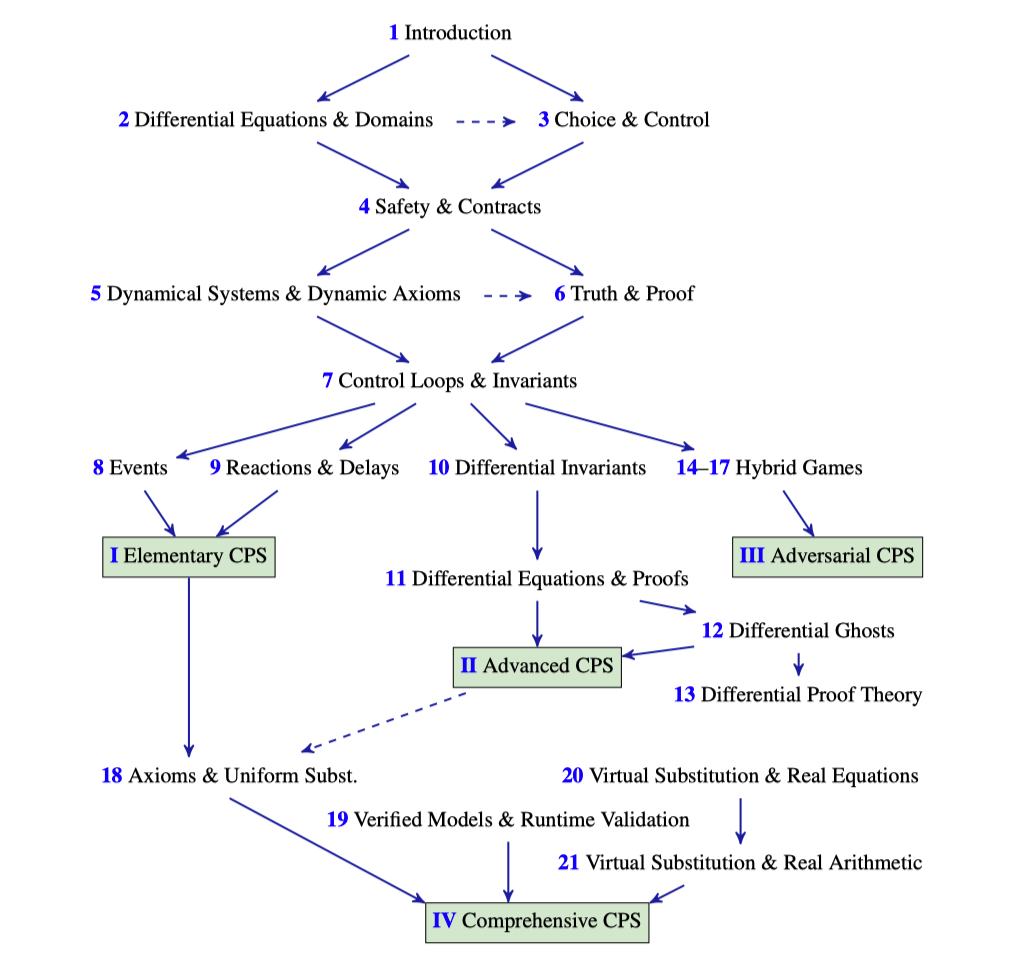
\includegraphics[width=.8\linewidth]{notes/hybridsystem/figures/structure-of-cps.png}
  \caption{Dependencies and suggested reading sequences}
  \label{fig:socps}
\end{figure}

\subsection{Differential Equations and Domains}

Differential equations are used to model the fundamental pieces of CPS.
\ctextit{They model processes in which the state variables of a system evolve continuously in time.}
It describes how the variables change locally, so it, basically, indicates the direction in which the variables evolve at each point in space.
These variables are presented in the \ctextbf{state space}.
For example, a car, which states can be denoted as a tuple $<x, v, a>$, 
is modeled by differential equations.
The $x$ is the position, $v$ is the velocity, and $a$ is the acceleration.
Hence, the car follows the equation:
\begin{align*}
  v = x' \text{, } a = v'
\end{align*}
In this case, the direction of $x$ is $v$, and the direction of $v$ is $a$.
Here the definition of ordinary differential equation is presented in Def. \ref{def:odequation}.
\clanewdef{Ordinary Differential Equation}{def:odequation}{
  Let $f: D \to \mathds{R}^n$ be a function on a $\text{domain } D \subseteq \mathds{R} \times \mathds{R}^n$, i.e., an open and connected subset.
  The function $Y: J \to \mathds{R}^n$ is a \textbf{solution} on interval $J \subseteq \mathds{R}$ of the \textbf{initial value problem}
  \begin{align*}
    &y'(t) = f(t, y) \\
    &y(t_0) = y_0
  \end{align*}
  with \textbf{ordinary differential equation (ODE)} $y' = f(t, y)$, 
  if, for all times $t \in J$: 
  (1) solution $Y$ is in the domain $(t, Y(t)) \in D$;
  (2) time-derivative $Y'(t)$ exists and is $Y'(t) = f(t, Y(t))$; and
  (3) initial value $Y(t_0)=y_0$ is respected at the initial time, also $t_0 \in J$.
}

To solve the equations, the infinite continuous line will be \ctextbf{discretized} into the finite discrete points.
If the equation is quite well behaved, the discretizations would approach the true continuous solutions as the $\Delta$ gets smaller.
However, no matter how small a discretization $\Delta > 0$ we choose, that discretization will be arbitrarily \ctextit{far away from the true continuous solution for large t}.

\begin{table}[h]
  \centering
  \caption{The differential equation examples}
  \vspace{0.5em}
  \begin{tabular}{c m{6cm} m{6cm}}
    \hline
    \thead{No.} & \thead{Name} & \thead{Differential Equation} \\
    \hline
    1 & A constant differential equation & $x'(t) = C_1, x(t_0) = C_2$ \\
    2 & A negative linear differential equation & $x'(t) = -C_1x(t), x(t_0) = C_2$ \\
    3 & A positive linear differential equation & $x'(t) = C_1x(t), x(t_0) = C_2$ \\
    4 & \ctextbf{Accelerated motion in a straight line} & $\begin{cases} x'(t) = v(t), x(0) = x_0 \\ v'(t) = a, v(0) = v_0 \end{cases}$ \\
    5 & \ctextbf{A two-dimensional linear differential equation for rotation} & $\begin{cases} v'(t) = w(t), v(0) = 0 \\ w'(t) = -v(t), w(0) = 1 \end{cases}$ \\
    6 & A similar two-dimensional linear differential equation for rotation & $\begin{cases} v'(t) = w(t), v(0) = 1 \\ w'(t) = -v(t), w(0) = 1 \end{cases}$ \\
    7 & \ctextbf{An adjustable linear differential equation for rotation} & $\begin{cases} v'(t) = \omega w(t), v(0) = 0 \\ w'(t) = -\omega v(t), w(0) = 1 \end{cases}$ \\
    8 & Time square oscillator & $\begin{cases} x'(t) = t^2 y(t), x(0) = 0 \\ y'(t) = -t^2 x(t), y(0) = 1 \end{cases}$ \\
    9 & Damped oscillator & $\begin{cases} x'(t) = y(t), x(0) = 1 \\ y'(t) = -4x(t)-0.8y(x), y(0) = 0 \end{cases}$ \\
    \hline
  \end{tabular}
  \label{tab:deexamples}
\end{table}

Here is a tiny compendium of differential equation examples shown in Tab. \ref{tab:deexamples}.
The solutions of a part of the equations are shown as follows:
\begin{align}
  &v(t) = sin(t), w(t) = cos(t) \text{, } \label{eq:deexp5} \\
  &v(t) = cos(t) + sin(t), w(t) = cos(t) - sin(t) \text{, } \label{eq:deexp6} \\
  &v(t) = sin(\omega t), w(t) = cos(\omega t) \text{, } \label{eq:deexp7} \\
  &x(t) = sin(\frac{t^3}{3}), y(t) = cos(\frac{t^3}{3}) \text{, } \label{eq:deexp8}
\end{align}
where Eq. \ref{eq:deexp5} corresponds to No. 5; 
Eq. \ref{eq:deexp6} corresponds to No. 6;
Eq. \ref{eq:deexp7} corresponds to No. 7;
Eq. \ref{eq:deexp8} corresponds to No. 8.

However, how physics and cyber elements interact?
To answer this question, we already know that physics does not literally stop evolving, but rather keeps on evolving all the time.
We can assume that the physics may pause for a period of duration 0 and lets the cyber take action to influence the inputs on which physics is based.
A chance should be given to the cyber elements to perform their task.
As a result, \ctextbf{evolution domain $Q$} is formally proposed (shown in Def. \ref{def:edconstraint}).
\clanewdef{Evolution domain constraint}{def:edconstraint}{
  A differential equation $x' = f(x)$ with \textbf{evolution domain Q} is denoted by
  \begin{align*}
    x' = f(x) \& Q
  \end{align*}
  using a conjunctive notation (\&) between the differential equation and its evolution domain.
  This notation $x' = f(x) \& Q$ signifies that the system obeys both the differential equation $x' = f(x)$ and the evolution domain $Q$. 
  The system follows this differential equation for \ctextit{any duration while inside the region $Q$}, 
  but is \ctextit{never allowed to leave} the region described by $Q$.
  So the system evolution has to stop while the state is still in Q.
}

Moreover, the cyber and the physics can interface in more than one way: 
(1) \footnote{The periodical runtime model}
\ctextit{the cyber elements interrupt physics periodically} to make measurements of the current state of the system in order to decide what to do next;
(2) \footnote{The event-driven runtime model}
\ctextit{the physics might trigger certain conditions or events} that cause cyber elements to compute their respective responses to these events.

